\documentclass{article}
\usepackage[a4paper, margin=1in]{geometry}
\usepackage{lipsum} % Для генерации фиктивного текста
\usepackage[T2A]{fontenc}
\usepackage{graphicx}


\begin{document}
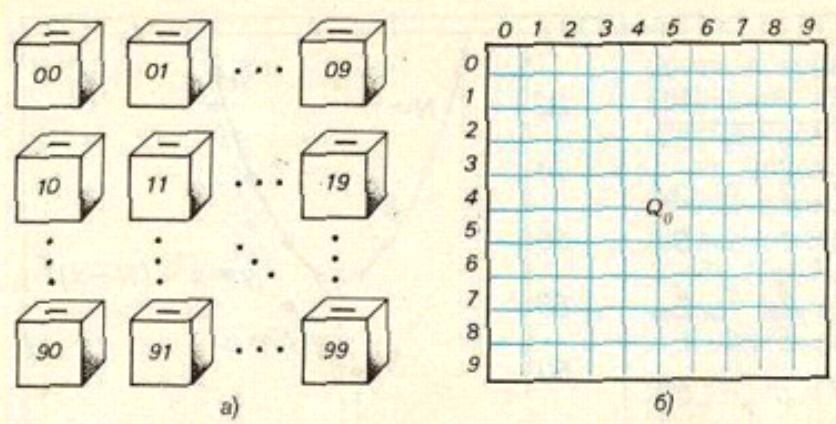
\includegraphics[width=10cm, height=5cm ]{6.png}
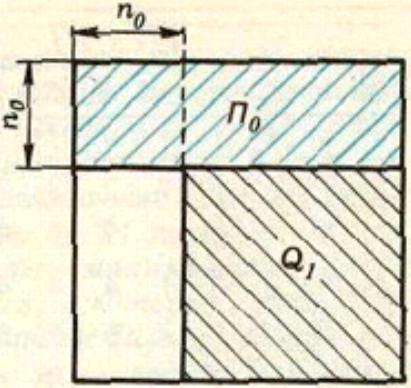
\includegraphics[width=5cm, height=5cm ]{7.png}

\vspace{0.5cm}

\begin{minipage}{0.45\textwidth}
\begin{flushleft}
Рис. 5.
\end{flushleft}
\newline
ток, а именно $n_0$, закрашено в нулевой строчке; можно считать, что это первые $n_0$ клеток строчки. Рассмотрим теперь квадрат $Q_{\mathrm{I}}$, получающийся из $Q_0$ вычеркиванием первых $n_0$ строчек и первых $n_0$ столбцов (рис. 6). Покажем, что все клетки $Q_1$ должны быть закрашены. Для этого возьмем ящики с номером $x y$, где $x \geqslant n_0$, $y \geqslant n_0$. В него обязательно попадает билет $0 x y$ : его нельзя положить в ящики $0 x$ и $0 y$, так как соответствующие клетки не закрашены. Значит, клетка с номером $x y$ должна быть закрашена для всех $x \geqslant n_0$, $y \geqslant n_0$.

Посчитаем, сколько же всего клеток закрашено в нашем квадрате $Q_0$. В каждой строчке прямоугольника $\Pi_0$ (см. рис. 6) закрашено по крайней мере $n_0$ клеток. В $Q_1$ закрашены все $\left(10-n_{\mathrm{n}}\right)^2$ клеток. Таким образом, в $Q_0$ закрашено по крайней мере $n_0^2+\left(10-n_0\right)^2$ клеток. Наименышая из этих сумм равна $F(2,10) 50$. Так что, во всяком случае, в $Q_0$ закрашено не менее 50 клеток. С другой стороны, пятидесяти ящиков с номерами, выписанными на рисунке 7, достаточно: вычеркнув в номере каждого билета цифру так, чтобы оставались две цифры одинаковой четности, мы поместим этот билет в соответствующий ящик. Эти два соображения завершают решение пунктов а) и в) задачи.
3. Решение задачи д)

Пусть теперь былеты $k$-значные. Будем считать, что у нас не 10 цифр, а $N$, где $N$ - некоторое произво.льное натуральное число (так, как если бы у
\end{minipage}
\hfill
\begin{minipage}{0.45\textwidth}
\begin{center}
    Рис. 6.
\end{center}

\newlineнас была принята $N$-ичная система счисления).
Строчки квадрата $Q_0$ занумеруем теперь числами от 0 до $N-1$; таким образом, в $Q_0$ всего $N^2$ клеток.
По-прежнему будем считать, что в нулевой строчке - $n_0$ закрашенных клеток, а в любой другой строчке не меньше, чем $n_0$. Аналогично построим квадрат $Q_1$. Поступим с $Q_1$ так же, как мы поступали с $Q_0$, выберем в нем строчку, в которой меньше всего закрашенных клеток (пусть это его первая строчка, т. е. строчка с номером $n_0$ в исходном квадрате), обозначим количество закрашенных клеток в ней через $n_1$ и, выкинув из $Q_1$ первые $n_1$ строчек и столбцов, получим квадрат $Q_2$. С ним поступим так же, и т. д., до квадрата $Q_{k-2}$ (рис. 8). Прямоугольники, аналогичные $\Pi_0$, обозначим через
\vspace{0.3} % Расстояние между таблицей и текстом
\begin{center}
\begin{tabular*}{\textwidth}{| @{\extracolsep{\fill}} |c|c|c|c|c|}
\hline 00 & 02 & 04 & 06 & 08 \\
\hline 11 & 13 & 15 & 17 & 19 \\
\hline 20 & 22 & 24 & 26 & 28 \\
\hline 31 & 33 & 35 & 37 & 39 \\
\hline 40 & 42 & 44 & 46 & 48 \\
\hline 51 & 53 & 55 & 57 & 59 \\
\hline 60 & 62 & 64 & 66 & 68 \\
\hline 71 & 73 & 75 & 77 & 79 \\
\hline 80 & 82 & 84 & 86 & 88 \\
\hline 91 & 93 & 95 & 97 & 99 \\
\hline
\end{tabular}
\end{center}
Рис. 7.
\end{minipage}


\end{document}
